% DEPRECATED FILE
\section{MaskD: Una Herramienta para Medir Masking-Tolerancia a Fallas}
\label{sec:maskD}

En esta sección presentamos {\MaskD}, una herramienta automática diseñada para medir el nivel de tolerancia a fallas entre componentes de software, 
descritos por medio de un lenguaje de comandos con guardas.
La herramienta se enfoca en medir componentes tolerantes a fallas de tipo enmascarante, es decir, programas que enmascaran fallas de tal manera que no puedan ser observadas por el ambiente. Usualmente se lo clasifica como el el tipo de tolerancia mas beneficioso y es a su vez una propiedad altamente deseable para sistemas críticos. 
La herramienta toma como entrada un modelo nominal y un modelo de su implementación tolerante a fallas y computa automáticamente la distancia de enmascaramiento entre ellos. 

La herramienta está diseñada para darle soporte a ingenieros de software para el análisis y diseño de sistemas tolerantes a fallas. Más precisamente, utiliza una función de distancia de enmascaramiento de tal forma que el ingeniero pueda medir la tolerancia enmascarante de una implementación tolerante a fallas dada, es decir, la cantidad de fallas que la implementación es capaz de enmascarar en el peor caso posible. 
Por lo tanto, los ingenieros pueden medir y comparar la distancia de tolerancia a fallas enmascarante entre distintas implementaciones y el modelo nominal, y así seleccionar la implementación que mejor se adapte a sus preferencias.

\subsection{La Herramienta} \label{sec:mask_sec}

\MaskD~toma como entrada un modelo nominal y su implementación tolerante a fallas, y produce como salida la distancia de enmascaramiento entre ellos, la cual es un valor en el intervalo $[0,1]$.
Los modelos de entrada se describen utilizando el lenguaje de comandos con guardas introducido en \cite{AroraGouda93}, un lenguaje de programación simple para describir algoritmos tolerantes a fallas.
Mas precisamente, un programa descrito en este lenguaje es una colección de procesos, donde cada proceso esta compuesto por una colección de acciones etiquetadas del estilo: $[Label]~Guard \rightarrow Command$, donde $Guard$ es una condición lógica sobre el estado actual del programa, $Command$ es una colección de asignaciones básicas que se ejecutan simultáneamente, y $Label$ es un nombre para la acción.
Estas construcciones sintácticas se denominan acciones. El lenguaje también permite a los usuarios etiquetar una acción como \emph{internal} (es decir, acciones silenciosas). Esto es importante para abstraerse de los mecanismos internos de el sistema que se modela y permitir construir modelos mas complejos. Además, algunas acciones pueden ser etiquetadas como \emph{faulty} para indicar que representan fallas. 

\begin{figure}[t]
\centering
\begin{minipage}[t]{.47\textwidth}
\fontsize{10}{10}\selectfont\ttfamily
\begin{tabbing}
x\=xxxxxxxx\=xxxxxxxxxxxx\=xx\=xxx\= \kill    
Process MEMORIA \{\\[1ex]
\>r : BOOL;  // valor observable \\ 
\>b0 : BOOL; // bit de memoria\\[1ex]
\>Initial: b0 \&\& r;\\[1ex]
%\>                   \>\>// 1 = refreshing\\[1ex]
\>[write1]  true -> b0=true, \\
\>\>~r=true; \\
\>[write0]  true -> b0=false, \\
\>\>~r=false; \\
\>[read0] !r -> r=r; // skip \\
\>[read1]  r -> r=r; // skip \\[1ex]
\}\\
\end{tabbing}
\end{minipage}
\caption{Modelo nominal para el ejemplo de la celda de memoria.} \label{fig:exam_1_mem_cell_nominal}
\end{figure}

\hfill

\begin{figure}[t]
\centering
\begin{minipage}[t]{.47\textwidth}
\fontsize{10}{10}\selectfont\ttfamily
\begin{tabbing}
x\=xxxxxxxx\=xxxxxxxxxxxxx\=xxx\=xxx\= \kill    
Process MEMORIA\_FT \{\\[1ex]
\>r : BOOL; // valor observable \\
\>b0 : BOOL; // primer bit \\
\>b1 : BOOL; // segundo bit \\
\>b2 : BOOL; // tercer bit \\[1ex]
%\>\textcolor{red}{f : [0..1] init 0;} \>\>\textcolor{red}{// fault limiting artifact}\\[1ex]
\>Initial: b0 \&\& b1 \&\& b2 \&\& r;\\[1ex]
\>[write1]  true -> b0=true, b1=true,  \\
\>\>~b3=true, r=true; \>\> \\
\>[write0]  true -> b0=false, b1=false,  \\
\>\>~b3=false, r=false; \>\> \\
\>[read0]  !r -> r=r; // skip \\
\>[read1]  r ->  r=r; // skip \\
\>[fault1]  faulty true -> b0=!b0, r =(!b0\&\&b1)||(b1\&\&b2)|| \\ 
\>\>(!b0\&\&b2); // el primer bit falla  \\
\>[fault2]  faulty true -> b1=!b1, r =(b0\&\&!b1)||(!b1\&\&b2)|| \\ 
\>\>(b0\&\&b2); // el segundo bit falla  \\
\>[fault3]  faulty true -> b2=!b2, r =(b0\&\&b1)||(b1\&\&!b2)|| \\ 
\>\>(b0\&\&!b2); // el tercer bit falla  \\[1ex]
\}\\
\end{tabbing}
\end{minipage}
\caption{Modelo con fallas para el ejemplo de la celda de memoria.} \label{fig:exam_1_mem_cell_faulty}
\end{figure}

Como ejemplo, consideremos la celda de memoria vista en el capitulo anterior. 
Un estado en este sistema mantiene el valor corriente de la celda de memoria ($m=i$, para $i=0,1$), la operación de escritura permite cambiar este valor, y la operación de lectura retorna el valor almacenado.  
En este sistema el resultado de una lectura dependerá del valor almacenado en la celda. 
Por lo tanto, una propiedad que uno podría asociar a este modelo es que el valor leído de la celda debe coincidir con el valor escrito por la ultima operación de escritura realizado por el sistema. 
    
Como se ha visto anteriormente, una falla potencial en este escenario ocurre cuando la celda pierde su carga de forma inesperada, y su valor almacenado cambia sin que se haya realizado una escritura (e.g., cambia de $1$ a $0$ por perdida de carga). Una técnica típica para lidiar con esta situación es el uso de \emph{redundancia}: 
en este caso, se utilizan tres bits de memoria en lugar de solo uno. Las operaciones de escritura son realizadas simultáneamente en los tres bits. 
La operación de lectura, por otro lado, retorna el valor que se repite al menos dos veces en los bits de memoria; esto se conoce como \emph{votación}. 
Las figuras \ref{fig:exam_1_mem_cell_nominal} y \ref{fig:exam_1_mem_cell_faulty} muestran los procesos representando el modelo nominal y el modelo de la implementación tolerante a fallas respectivamente para este ejemplo. 

\subsection{Arquitectura}

\MaskD~es software de código abierto escrito en el lenguaje \textsf{Java}. La documentación y las instrucciones de instalación se pueden encontrar en \cite{MaskD}. La arquitectura de la herramienta se muestra en la figura~\ref{fig:arch}.
\begin{figure}[t]
    \centering
    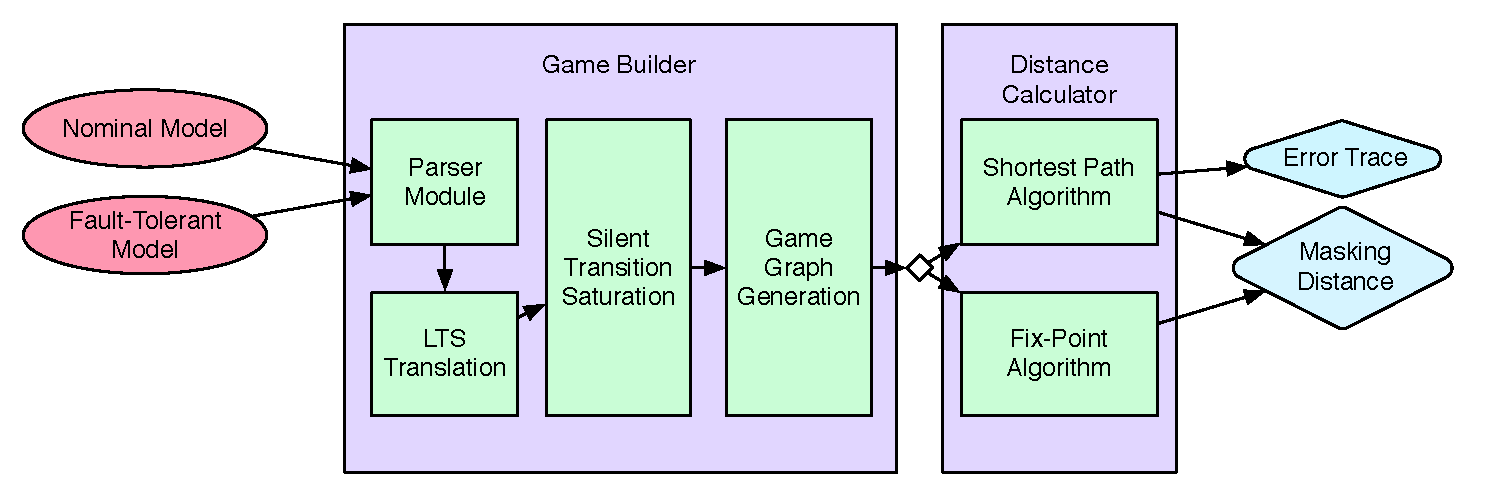
\includegraphics[scale=0.50]{Figs/architecture-eps-converted-to.pdf}
    \caption{Arquitectura de \textsf{MaskD}.}\label{fig:arch}
\end{figure}
    Discutiremos brevemente las componentes principales de la herramienta:
\begin{description}
    \item[Módulo Parser.] Realiza análisis sintáctico básico sobre los modelos de entrada y produce estructuras de datos que representan a  estas entradas. Para esto se utilizan las bibliotecas \textsf{Cup} y 
    \textsf{JFlex} para generar automáticamente el parser a partir de la gramática que describe el lenguaje de modelado.
    \item[Traducción a LTS.] Los modelos obtenidos del parser son traducidos a Sistemas de Transición Etiquetados (LTS), es decir, 
    grafos donde los vértices representan estados del programa y donde las transiciones mantienen información sobre las acciones de los modelos. 
    \item[Saturación de Transiciones Silenciosas.] Las transiciones internas/silenciosas en los LTS que representan los modelos de entrada son saturadas utilizando algoritmos estándar que provienen de teoría sobre álgebras de procesos \cite{Milner89}. Como resultado, se generan LTS saturados, estos son necesarios para verificar la relación de enmascaramiento cuando existen transiciones internas.
    \item[Generación del Grafo de Juego.] Utiliza los LTS saturados para producir un grafo de juego. Los nodos en este grafo codifican la configuración corriente del juego: 
    el próximo jugador que debe jugar, la ultima acción jugada, y referencias a los estados de los LTS de los modelos de entrada que se corresponden con la configuración actual del juego. 
    Las transiciones en este grafo corresponden a las posibles jugadas para los jugadores, es decir,  transiciones en los LTS originales.
    \item[Algoritmo de Camino mas Corto.] Si los modelos de entrada son deterministas en las etiquetas de sus acciones, el algoritmo de camino mas corto de Dial es utilizado para obtener el camino mas corto hacia el estado de error, desde el cual se calcula el valor final.
    \item[Algoritmo de Punto Fijo.] Este es el algoritmo por defecto, funciona tanto para modelos deterministas como no deterministas en las etiquetas de sus acciones, utiliza una búsqueda de estilo \textit{bottom-up breadth-first} para computar el valor del juego. 
    Este algoritmo se basa en algoritmos conocidos para resolver juegos de alcanzabilidad que utilizan conjuntos \emph{atractores} \cite{Jurd11}. 
    %This algorithm is polynomial in the game graph size.
\end{description}
Como se ha explicado mas arriba, un punto interesante sobre la herramienta es que, para sistemas deterministas en sus acciones, la distancia de enmascaramiento entre dos sistemas puede ser computada recurriendo al algoritmo de camino mas corto de Dial \cite{Dial69}, el cual tiene complejidad lineal con respecto al tamaño de los grafos utilizados para representar los sistemas.
En el caso de los sistemas no deterministas, se necesita un recorrido con punto fijo, lo cual hace que el algoritmo sea menos eficiente. Sin embargo, aun en este caso sigue siendo polinomial. 

%TODO: draw architecture and explain

%In order to measure the degree of masking fault-tolerance of a given system, 
%we start characterizing masking fault-tolerance via simulation relations between 
%two systems as defined in \cite{DemasiCMA17}. 
%The first one acting as a specification 
%of the intended behavior (es decir, nominal model) and the 
%second one as the fault-tolerant implementation (es decir, the extended model with 
%faulty behavior).
%The existence of a masking relation implies that the implementation masks the faults.
%Afterwards, we introduce a game characterization of 
%masking simulation and we enrich the resulting games 
%with quantitative objectives to define the notion of 
%\emph{masking fault-tolerance distance}, 
%where the possible values of the game belong to the interval $[0,1]$. 

\subsection{Modo de Uso}

El comando estándar para ejecutar {\MaskD} en un sistema operativo de estilo Unix es:
\\ 
\\
 \verb"./MaskD <options> <spec_path> <imp_path>"
\\
\\
En este caso la herramienta arroja como resultado la distancia de masking entre la especificación y la implementación utilizando el algoritmo por defecto (algoritmo de punto fijo).
Algunos comandos opcionales incluyen: \verb"-t: print error trace", el cual muestra por salida estándar una traza hasta el estado de error bajo estrategias óptimas; y  \verb"-s: start simulation", el cual comienza una simulación manual desde el estado inicial.  
Obtener un camino hacia el estado de error es una funcionalidad útil para encontrar defectos en las descripciones de programas, los cuales pueden fallar por razones no intencionales. A su vez la traza sirve para ver como se comportan las estrategias óptimas de los jugadores. Una traza para el ejemplo de la celda de memoria se muestra en la figura~\ref{fig:trace_mem_cell}. Los estados se muestran en el formato \verb"{spec_state, last_action_played, imp_state, player_turn}", donde \verb"spec_state" es el estado corriente del modelo nominal, \verb"last_action_played" es la última acción que se jugó (solo es relevante para estados del Verificador), \verb"imp_state" es el estado del modelo que representa a la implementación y \verb"player_turn" es el jugador cuyo turno corresponde jugar. En este caso, después de dos fallas (bits que cambian de valor sin que haya una escritura), al luego realizar una lectura, nos lleva al estado de error ya que en el modelo nominal el valor de la celda es $0$, mientras que el el modelo tolerante a fallas el valor leído en la mayoría (votación) de bits es $1$. Por otro lado, la funcionalidad de simulación permite al usuario seleccionar manualmente las acciones disponibles en cada punto del juego de enmascaramiento, lo cual también es útil para verificar que los modelos se comportan como el usuario espera.
Por defecto, \MaskD~computa la distancia de enmascaramiento para una entrada dada utilizando el algoritmo para sistemas no deterministas. 
El usuario puede utilizar la opción \verb"-det" para cambiar al algoritmo de distancia de enmascaramiento para sistemas deterministas.
\begin{figure}[t]
\centering
\begin{minipage}[t]{.47\textwidth}
\fontsize{10}{10}\selectfont\ttfamily
\begin{tabbing}
0. \{ <mr,mb0> , \# , <mr,mb0,mb1,mb2> , R \} \\ 
1. \{ <mr,mb0> , I\_m.fault1 , <mr,mb1,mb2> , V \} \\ 
2. \{ <mr,mb0> , \# , <mr,mb1,mb2> , R \} \\ 
3. \{ <mr,mb0> , I\_m.fault2 , <mb2> , V \} \\ 
4. \{ <mr,mb0> , \# , <mb2> , R \} \\ 
5. \{ <mr,mb0> , S\_m.read1 , <mb2> , V \} \\ 
6. ERR\_STATE \\ 
\end{tabbing}
\end{minipage}
\caption{Traza de Error para el ejemplo de la celda de memoria.} \label{fig:trace_mem_cell}
\end{figure}


\subsection{Evaluación Experimental} \label{sec:experimental_eval}
%\subsection{Details of the implementation}

%Las técnicas descritas en el capitulo anterior fueron implementadas en una herramienta utilizando el lenguaje \textsf{Java}, la herramienta se llama \MaskD: 
%Masking Distance Tool \cite{MaskD}. 
%\MaskD~ toma como entrada un modelo nominal y su implementación tolerante a fallas, 
%y produce como salida la distancia de masking entre ellos. 
%Los modelos son especificados utilizando el lenguaje de guardas introducido en \cite{AroraGouda93}, un lenguaje de programación simple comúnmente utilizado para describir algoritmos tolerantes a fallas.
%Mas precisamente, un programa es una colección de procesos, donde cada proceso está compuesto de una colección de acciones del estilo: $Guard \rightarrow Command$, donde $Guard$ es una condición lógica sobre el estado actual del programa y $Command$ es una colección de asignaciones básicas. Estas construcciones sintácticas se denominan acciones. El lenguaje también permite al usuario etiquetar una acción como interna (es decir, acciones $\tau$). Además, lagunas acciones pueden representar fallas en el sistema.
%La herramienta posee varias funcionalidades extra como por ejemplo mostrar trazas hacia el estado de error o iniciar una simulación desde el estado inicial.

En la Tabla~\ref{table:results} reportamos los resultados de la distancia de masking para múltiples instancias de varios casos de estudio. Estos incluyen: una Celda de Memoria Redundante (nuestro ejemplo motivador), Redundancia N-Modular (un ejemplo estándar de sistemas tolerantes a fallas \cite{ShoomanBook}), una variación del problema de los Filósofos Comensales \cite{Dijkstra71}, el problema de los Generales Bizantinos introducido por Lamport et al. \cite{LamportSP82}, una prueba de consistencia de parte del algoritmo de consenso Raft \cite{OngaroO14}, y el Protocolo de Retransmisión Acotada (un ejemplo bien conocido de un protocolo tolerante a fallas \cite{GrooteP96}). Todos los casos de estudio han sido evaluados utilizando los algoritmos para juegos deterministas y no deterministas (columnas ``Tiempo'' y ``Tiempo(Det)'', respectivamente), con la excepción de los modelos netamente no deterministas (por ejemplo, el problema de los Generales Bizantinos y el Protocolo de Retransmisión Acotada). Es de destacar que la complejidad computacional yace principalmente en la construcción explícita del grafo de juego y no del cálculo de la distancia de masking en si.

A continuación se da una interpretación de los resultados experimentales. Para el caso de una memoria redundante de $3$ bits, la distancia de masking es $0.333$. El principal motivo de esto es que el modelo con fallas, en el peor caso, solo es capaz de enmascarar $2$ fallas (en este ejemplo, una falla representa un cambio inesperado en el valor de un bit, posiblemente por una descarga) antes de fracasar al tratar de replicar el comportamiento del modelo nominal (es decir leer el valor votado por la mayoría). Por lo tanto, el resultado viene de la definición de distancia de masking y de tener en cuenta la ocurrencia de dos fallas. La situación es similar para otras instancias de este problema con mas redundancia de bits.

La Redundancia N-Modular consiste de N sistemas, los cuales desarrollan una tarea o proceso y que los resultados son procesados por un sistema de votación de mayoría para producir una única salida. 
Asumiendo un único votante perfecto, hemos evaluado este caso de estudio para diferentes cantidades de módulos.
%Note that, in this case study, the distance measuring exhibits a similar pattern to that of the 
Note que las medidas de distancia para este caso son similares al de la memoria redundante. 

\begin{table} [ht!]
\centering
\setlength{\tabcolsep}{7pt}
    \scalebox{0.85}{
  \begin{tabular}{c c c c c} \toprule
    Case de Estudio      & Redundancia & D.Masking & Tiempo & Tiempo(Det)  \\ \midrule
    \multirow{5}{*}{Celda de Memoria}          & $3$ bits & $0.333$ & $0.7$\text{s} & $0.6$\text{s}\\
                & $5$ bits & $0.25$ & $2.5$\text{s} & $1.9$\text{s}\\
                & $7$ bits & $0.2$ & $7.2$\text{s}  & $5.7$\text{s}\\
                & $9$ bits & $0.167$ & $1m.4s$ & $1$\text{m}$11$\text{s}\\
 		 	    & $11$ bits & $0.143$ & $28m27s$ & $26$\text{m}$10$\text{s}\\ \midrule
    \multirow{5}{*}{Redundancia N-Modular}           & $3$ módulos & $0.333$ & $0.6$\text{s} & $0.5$\text{s} \\
                & $5$ módulos & $0.25$ & $1.2$\text{s} & $0.7$\text{s}\\
                & $7$ módulos & $0.2$ & $5.6$\text{s}  & $3.8$\text{s}\\ 
                & $9$ módulos & $0.167$ & $2$\text{m}$55$\text{s}  & $2$\text{m}$32$\text{s}\\
 		 	    & $11$ módulos & $0.143$ & $75$\text{m}$17$\text{s}  & $72$\text{m}$48$\text{s}\\ \midrule
    \multirow{5}{*}{Filósofos Comensales}    & $2$ filósofos & $0.5$ & $0.6$\text{s} & $0.6$\text{s}\\
	            & $3$ filósofos & $0.333$ & $1.9$\text{s} & $0.9$\text{s}\\
	            & $4$ filósofos & $0.25$ & $5.9$\text{s} & $2.6$\text{s}\\ 
				& $5$ filósofos & $0.2$ & $25.3$\text{s} & $24.1$\text{s}\\ 
				& $6$ filósofos & $0.167$ & $19$\text{m}$23$\text{s} & $11$\text{m}$39$\text{s}\\ \midrule
    \multirow{3}{*}{Generales Bizantinos}    
                & $3$ generales & $0.5$ & $0.9$\text{s} & $-$ \\
            	& $4$ generales & $0.333$ & $17.1$\text{s} & $-$\\ 
            	& $5$ generales & $0.333$ & $429$\text{m}$54$\text{s} & $-$\\ \midrule
    \multirow{3}{*}{Raft LRCC (5)}        & $1$ seguidor & $0$ & $0.7$\text{s} & $0.8$\text{s}\\
            & $2$ seguidores & $0$ & $5.6$\text{s} & $3.6$\text{s} \\ 
            & $3$ seguidores & $0$ & $49$\text{m}$50$\text{s} & $37$\text{m}$53$\text{s} \\ \midrule
    \multirow{5}{*}{BRP(1)}       	& $1$ retransm. & $0.333$ & $0.7$\text{s} & $-$\\ 
 						& $5$ retransm. & $0.143$ & $0.8$\text{s}  & $-$\\ 
 						& $10$ retransm. & $0.083$ & $1.3$\text{s}  & $-$\\ 
 						& $20$ retransm. & $0.045$ & $3.9$\text{s}  & $-$\\ 
 						& $40$ retransm. & $0.024$ & $4.8$\text{s} & $-$ \\ \midrule
	\multirow{5}{*}{BRP(5)}       	& $1$ retransm. & $0.333$ & $4.2$\text{s} & $-$\\
					& $5$ retransm. & $0.143$ & $4.8$\text{s}  & $-$\\ 
					& $10$ retransm. & $0.083$ & $6.1$\text{s}  & $-$\\ 
					& $20$ retransm. & $0.045$ & $8.7$\text{s}  & $-$\\ 
					& $40$ retransm. & $0.024$ & $18.6$\text{s} & $-$ \\ \midrule
	\multirow{5}{*}{BRP(10)}       	& $1$ retransm. & $0.333$ & $4.7$\text{s} & $-$\\ 
					& $5$ retransm. & $0.143$ & $6.4$\text{s} & $-$ \\ 
					& $10$ retransm. & $0.083$ & $10.1$\text{s} & $-$ \\
					& $20$ retransm. & $0.045$ & $20.5$\text{s} & $-$ \\ 
					& $40$ retransm. & $0.024$ & $1$\text{m}$9$\text{s} & $-$ \\ \bottomrule
  \end{tabular}}
\vspace{0.2cm}
\caption{Resultados de la distancia de masking para los casos de estudio.}
\vspace{-0.8cm}
\label{table:results}
\end{table} 

Para el problema de los filósofos comensales, adaptamos la implementación par/impar en la cuál algunos filósofos obtienen primero el tenedor derecho y otros obtienen primero el izquierdo. Específicamente tenemos $n-1$ filósofos \emph{impares} que obtienen el tenedor derecho primero, y $1$ filósofo \emph{impar} que obtiene primero el izquierdo. En este caso, consideramos que ocurre una falla cuando un filósofo impar actúa como uno par, esto se puede entender como una falla bizantina. Para dos filósofos la distancia de masking es $0{.}5$ ya que basta con una falla para alcanzar un estado de deadlock. Mientras mas filósofos la distancia de masking se vuelve mas pequeña. 
%We have evaluated this problem on four instances with $2, 3, 4,$ and $5$ philosophers, respectively.

%\hrmkPRD{Explicar el de los Generales Bizantinos!!}
Otro ejemplo interesante de un sistema tolerante a fallas es el problema de los generales bizantinos, introducido originalmente por Lamport et al. \cite{LamportSP82}. Este es un problema de consenso, donde hay un general comandante con $n-1$ tenientes. La comunicación entre el general y sus tenientes ocurre a través de mensajeros. El general puede decidir entre atacar la ciudad enemiga o retirarse; luego, manda la orden a sus tenientes. Algunos de estos pueden ser traidores. 
Asumimos que los mensajes son entregados sin problemas y que todos los tenientes pueden comunicarse entre si de forma directa. Bajo este escenario ellos pueden reconocer quien mandó un mensaje. Las fallas pueden convertir a un teniente leal en un traidor (fallas bizantinas). En consecuencia, los traidores pueden mandar mensajes falsos o incluso omitir mandar los mensajes que recibieron a otros tenientes. Los tenientes leales deben acordar atacar o retirarse después de $m + 1$ rondas de comunicación, donde $m$ es el máximo número de traidores. Aquí consideramos el caso de $m=1$.  

%The algorithm can ensure correct operation only if fewer than one third of the lieutenants are traitors.

Raft \cite{OngaroO14} es un algoritmo de consenso que se ha vuelto popular en años recientes. En Raft, un líder es elegido de un conjunto de servidores disponibles, una vez electo, el líder recibe peticiones de clientes y las reenvía a sus seguidores (los demás servidores), así pueden replicar la información nueva en sus estados respectivos. Cada servidor mantiene un historial de las entradas recibidas. Un seguidor puede rechazar una entrada si existe alguna inconsistencia entre su historial y el historial del líder, esto se considera una falla en nuestro contexto. Cuando esto ocurre, el líder intenta nuevamente con la entrada anterior de su historial, esto se repite hasta que sea congruente con la entrada mas reciente del seguidor en conflicto. Aquí modelamos solo una de las etapas del algoritmo Raft, la etapa de Replicación de Historial. Específicamente, adaptamos el control de consistencia que realiza el protocolo para asegurar consistencia entre los historiales de los seguidores y el historial del líder. Computamos la distancia de masking para este modelo con $1$, $2$ y $3$ seguidores, y considerando un historial del líder de $5$ entradas. Notemos que esta distancia es siempre $0$. Intuitivamente, esto ocurre porque, a pesar de que puede haber rechazos, eventualmente todos los historiales van a estar de acuerdo (en el peor caso, el protocolo va a descartar todas las entradas de los seguidores hasta alcanzar un historial vacío, y luego copiarán todas las entradas del historial del líder en sus respectivos historiales). 

El Protocolo de Retransmisión Acotada o Bounded Retransmission Protocol (BRP) es un caso de estudio sobre verificación de software conocido en el ámbito industrial. Mientras los demás casos de estudio han sido tratados como "ejemplos de juguete" y analizados con $\DeltaMask$, el BRP fue modelado de forma mas cercana a una implementación siguiendo~\cite{GrooteP96}, considerando diferentes componentes (emisor, receptor, y canales). Para analizar tal modelo utilizamos la distancia de masking débil $\DeltaMask^W$.
Hemos calculado la distancia de masking para el protocolo con $1$, $5$ y $10$ trozos de mensaje a enviar, denotados BRP(1), BRP(5) y BRP(10), respectivamente. 

Podemos observar que los valores de la distancia no son afectados por la cantidad de trozos a enviar por el protocolo. Esto es de esperar, debido a que la distancia de masking depende de la redundancia agregada para enmascarar fallas, en este caso, depende de la cantidad de retransmisiones permitidas.

Los experimentos fueron realizados en una MacBook Air con un procesador Intel Core i5 de 1.3 GHz y una memoria RAM de 4GB. El código fuente y los archivos ejecutables de la herramienta así como los casos de estudio para reproducir los resultados se encuentran disponibles en un repositorio Github \cite{MaskD}.




